\documentclass[output=paper]{langsci/langscibook}
\ChapterDOI{10.5281/zenodo.1182593}
\author{Patrick Hanks\affiliation{RIILP, University of Wolverhampton, England}%
\and Ismail El Maarouf\affiliation{Adarga Ltd., England}%
\lastand Michael Oakes\affiliation{RIILP, University of Wolverhampton, England}}
\title{Flexibility of multiword expressions and Corpus Pattern Analysis}

\abstract{This chapter is set in the context of \isi{Corpus Pattern Analysis} (CPA), a technique developed by Patrick Hanks to map meaning onto word patterns found in corpora. The main output of CPA is the Pattern Dictionary of \ili{English} Verbs (PDEV), currently describing patterns for over 1,600 verbs, many of which are acknowledged to be multiword expressions (MWEs) such as phrasal verbs or idioms. PDEV entries are manually produced by lexicographers, based on the analysis of a substantial sample of concordance lines from the corpus, so the construction of the resource is very time-consuming. The motivation for the work presented in this chapter is to speed up the discovery of these word patterns, using methods which can be transferred to other languages. 
This chapter explores the benefits of a detailed contrastive analysis of MWEs found in English and \ili{French} corpora with a view on English-French translation. The comparative analysis is conducted through a case study of the pair (\textit{bite}, \textit{mordre}), to illustrate both CPA and the application of statistical measures for the automatic extraction of MWEs. The approach taken in this chapter takes its point of departure from the use of statistics developed initially by \cite{church1989}. Here we look at statistical measures which have not yet been tested for their ability to discover new collocates, but are useful for characterizing verbal MWEs already found. In particular we propose measures to characterize the mean span, rigidity, diversity, and idiomaticity of a given MWE.}

\maketitle

\begin{document}

\section{Introduction: phraseology and Multi-Word Expressions}

\is{meaning|(}
Traditionally, people have long believed that each word has one or more
meanings and that these meanings can be selected and put together, as
if in a child’s Lego set, to construct propositions, questions, etc.
This belief is still widely (and unquestioningly, unthinkingly) held by
many NLP (Natural Language Processing) researchers among others. This
may indeed be a good way of accounting for basic
\textit{propositional}
\textit{logic}, but it accounts at best for only a
very limited subset of natural language use. An alternative view is
that logics are by-products of natural language. At the very least, we
may say that the relationship between language and logic is not well
understood. If the “Lego set” theory of meaning in language were
tenable, it would not have been necessary for NLP and AI (Artificial
Intelligence) researchers such as \cite{ide2006}, after many
years of intensive (and expensive) effort, to declare that projects in
\isi{Word Sense Disambiguation } (WSD) have failed to achieve even their most
basic goals.


\begin{quotation}
At present, WSD work is at a crossroads: systems have hit a reported
ceiling of 70\%+ accuracy \citep{article}, the source and
kinds of sense inventories that should be used in WSD work is an issue
of continued debate, and the usefulness of stand-alone WSD systems for
current NLP applications is questionable. (\citealt[15]{ide2006}).
\end{quotation}


The alternative view mentioned here is supported by lexicographers such
as \cite{Atkins:2001}, \cite{article},  and \cite{hanks2000}.
These lexicographers argue that much of the meaning of an utterance is
carried by underlying patterns of co-selection of the words actually
used, rather than by simple concatenations. These conclusions overlap
to some extent with the tenets of \is{Construction Grammar} Construction Grammar, though the
methodologies are very different. In corpus linguistics, Sinclair
declared, after a lifetime’s empirical research into texts, corpora,
and meaning, “Many if not most meanings require the presence of more
than one word for their normal realisation” \citep[4]{sinclair1998}.

\is{meaning|)}

If these lexicographers and corpus linguists are right, it might appear
that MWEs play a central role in the meaningful use of language. They
are not merely an irritating set of exceptions, as used to be thought.
According to this, MWEs are not exceptions to the rule; they are the
rule. The exceptions, insofar as they exist in normal language use, are
isolated meaningful uses of single words.



It has long been obvious that the meaning of MWEs such as \textit{of course},
\textit{a ball-park figure}, and \textit{spill the beans} is not compositional. No
courses, ball parks, or beans are invoked by someone deconstructing the
meaning intended by a speaker who uses these expressions. However,
extended analysis of large volumes of data leads to the somewhat
unwelcome conclusion that the concept of a MWE may also be flawed,
being nothing more than an attempt to extend the ``Lego-set’' theory to
  cover some so-called \textit{fixed expressions} \is{multiword expression!fixed expression} such as \textit{spill the beans} and
\textit{kick the bucket}. Here, the choice of lexical items is fixed: one
cannot talk meaningfully, except perhaps in jest, about \textit{*tipping over
the haricots} or \textit{*booting the pail}. However, even in these very fixed
MWEs, certain grammatical alternations, in particular verb inflections,
are normal and unremarkable.



More to the point is the fact that many other expressions, that at first
sight might be considered compositional, are associated with a limited
phraseology. They do not vary freely, but employ selectional variations
drawn from within a (usually quite small) lexical set. Such patterns
are found for many expressions that intuitions alone might encourage us
to classify as fixed. Corpus evidence shows that people not only grasp
at straws, they also clutch at straws and even seize on straws. \cite{moon1998} observes that \textit{shiver in one’s shoes} (meaning `to be afraid') may
at first seem to be a fixed expression, but in fact corpus evidence
shows that every lexical item in the expression allows a modicum of
variation: people quake in their boots, shake in their sandals, and she
even found a mention of policemen quaking in their size fourteens.
(English policemen are supposed proverbially to have big feet.) The
meaning of the idiom is the same in all cases; the cognitive values of
the lexical items are so similar as to be virtually identical; and yet
the actual words used to realize the expression can be different. 


Conversely, when we examine the corpus evidence for an expression that
might uncontroversially be classified as compositional, such as (\ref{ex0}), 


\ea
\label{ex0}
\textit{the wind was blowing from the north}
\z



\noindent we find that the utterer of this unremarkable little sentence is in fact
activating the meaning by drawing on a pattern containing a small but
open-ended lexical set of items alternating with \textit{wind}: \textit{gale},
\textit{blizzard}, \textit{hurricane}, \textit{typhoon}, \textit{breeze}, \textit{air}, not to mention adjectival
subclassifications such as \textit{a hot dry wind}, \textit{a cold wind}, \textit{strong winds},
\textit{the fenland winds}, \textit{a unidirectional wind}. To these can be added some
much rarer lexical items such as \textit{tempest}, \textit{trades}, and \textit{zephyr}. At the
other end of the sentence forming the prototype or stereotype for this
particular pattern, we find a very much larger set of expressions
functioning as adverbials of direction: \textit{from the north}, including
\textit{from the south}, \textit{from the sea}, \textit{over a cliff face}, \textit{up the street}, \textit{through
a spider’s web}, and so on. 



These very conventional expressions are best classified as realizations
of non-compositional patterns \is{pattern} rather than as compositional
concatenations for a variety of reasons. A prominent one is that the
pattern so identified is contrastive: it is a set of stereotypical
phrases that contrast with other uses of the words. For example, this
pattern (see example \ref{ex1}) contrasts with other patterns having different
meanings formed with the same verb, such as \textit{to blow a whistle} and \textit{to
blow up a bridge}. 



Another reason for seeking to identify patterns of verb use is that,
once a pattern is established in the language or in the mind of a
speaker, it can be exploited metaphorically and in other ways. Some
typical exploitations of this pattern of the verb \textit{blow}, found in the
British National Corpus, \mbox{are shown in examples (\ref{ex1})-(\ref{ex5})}.



\ea
\label{ex1}
 \textit{Dennis Healey $[$a politician$]$ wobbles about according to which way
the wind is blowing.} 
\ex \label{ex2}
\textit{The winds of neo-liberalism are blowing a gale through Prague.}
\ex \label{ex3} 
\textit{Faint liberal breezes had been blowing through the Vatican since the
  second Vatican Council.}
\ex \label{ex4}  
\textit{\ldots the winds of change that have blown through the energy business.}
\ex \label{ex5} 
\textit{The winds of fate blew for Jean Morris, winner of Middlesbrough
Council's Captain Cook Birthday Balloon Race.}
\z






Metaphorical exploitations bring in additional evidence that a pattern
has become established. In the previous examples, the meaning can only
be understood in relation to the \textit{the wind blows} (not, say, \textit{blowing
up a bridge}), but cannot be confused with it, as there is no wind
blowing literally.



The aim of this short introduction to MWEs was to set the study of MWEs
in the broad context of phraseology, and stress the obstacles in the
way of linguistic description. In order to understand and process
meaning in text, it is necessary first to compile inventories of
patterns of language use, which can be used as benchmarks against which
actual utterances can be compared. The following section presents
Corpus Pattern Analysis, a method for deriving patterns from corpora.


\section{The Corpus Pattern Analysis framework}


\isi{Corpus Pattern Analysis}  (CPA) is a research procedure designed to create
empirically well-founded resources for NLP applications by combining
interactively human data analysis and machine learning. It is based on
the Theory of Norms and Exploitations (TNE, \citealt{hankspustejovsky2004}; \citealt{hanks2005}; \citealt{hanks2013}). 
%}~and~\href{http://pdev.org.uk/#biblio?id=hanks_2013}{2013},~\href{http://pdev.org.uk/#biblio?id=hanks_pustejovsky_2005}{Hanks
%\& Pustejovsky 2005}).
TNE in turn is a theory that owes much to the
work of Pustejovsky on the Generative Lexicon \citep{pustejovsky1995},
%(~\href{http://pdev.org.uk/#biblio?id=pustejovsky_1995}{Pustejovsky1995})
 to \cite{wilks1975}'s theory of preference semantics,
%(~\href{http://pdev.org.uk/#biblio?id=wilks}{Wilks 1975})
 to
Sinclair's work on corpus analysis and collocations (\citealt{Sinclair:66, sinclair1987, Sinclair:1991, sinclair2004}),
%Sinclair~\href{http://pdev.org.uk/#biblio?id=sinclair_1966}{1966},
%\href{http://pdev.org.uk/#biblio?id=sinclair_1987}{1987},~\href{http://pdev.org.uk/#biblio?id=sinclair_1991}{1991},~\href{http://pdev.org.uk/#biblio?id=sinclair_2004}{2004}),
to the Cobuild project in lexical computing \citep{sinclair1987}, 
%(\href{http://pdev.org.uk/#biblio?id=sinclair_1987}{Sinclair et al. 1987}), 
and to the Hector project (\citealt{atkins1992}; \citealt{hanks1994}).
%(\href{http://pdev.org.uk/#biblio?id=atkins_1993}{Atkins
%1993};~\href{http://pdev.org.uk/#biblio?id=hanks_1994}{Hanks 1994}).
CPA is also influenced by frame semantics \citep{Fillmore1992risk}. 
%(\href{http://pdev.org.uk/#biblio?id=fillmore_1992}{Fillmore \&
%Atkins 1992}). 
It is complementary
to FrameNet.
%~\href{http://framenet.icsi.berkeley.edu/}{FrameNet}.
Where FrameNet
offers an in-depth analysis of semantic frames, CPA offers a systematic
analysis of the patterns of meaning and use of each verb. Each CPA
pattern can in principle be plugged into a FrameNet semantic frame. Some
work in American linguistics \citep{jackendoff2002foundation}  has complained
about the excessive ``syntactocentrism" of American linguistics in the
20th century. TNE offers a lexicocentric approach, with opportunities
for synthesis, which will go some way towards redressing the balance.



CPA starts from the observation that whereas most words are very
ambiguous, most patterns have one and only one sense. Each word is
associated with a number of patterns based on valency, which is
comparatively stable, and one or more sets of preferred collocations,
which are highly variable \citep{hanks2012}.  In CPA, patterns of word use
are associated with statements of meaning, called \textsc{implicatures}. Each
pattern has a primary implicature (the meaning of the pattern), and
possibly a number of secondary implicatures \citep{deschryver2010}. To
take a simple example, the word \textit{blow} is multiply ambiguous. However,
the expression  \textit{blow your nose} is unambiguous and contrasts with 60 or
70 other patterns of use of the same verb.



In the \is{Pattern Dictionary of English Verbs} Pattern Dictionary of English Verbs (PDEV;
\url{http://pdev.org.uk}), the main output of CPA, the sense of  \textit{blow
  your nose} is stored in the pattern “[[Human]] blow \{nose\}” while in
the sense of “the wind blows” is represented by the pattern “$[$$[$Wind |
Vapour | Dust$]$$]$ blow $[$No object$]$ $[$Adverbial of direction$]$”. Patterns \is{pattern}
may combine various kinds of categories such as semantic types (Human,
Wind, Vapour, Dust), grammatical categories (Adverbial of direction)
and lexical items (\textit{nose}). Semantic types are taken from the
corpus-driven CPA Semantic Ontology available at
\url{http://pdev.org.uk/#onto}. These categories may fill slots in the
pattern template based on the SPOCA model, an acronym standing for the
main clause roles that may be filled by arguments of a verb in a
proposition: a Subject, a Predicator, an Object, a Complement, and an
Adverbial (Halliday 1994). Each argument can in turn be further
characterized if the pattern requires it, by filling information on the
``subargumental cues" such as the nature of determiners, modifiers,
quantifiers, prepositional phrases, and adverbs or particles.

\begin{figure}
%\includegraphics[width=\textwidth]{figures/img_04_01.png}
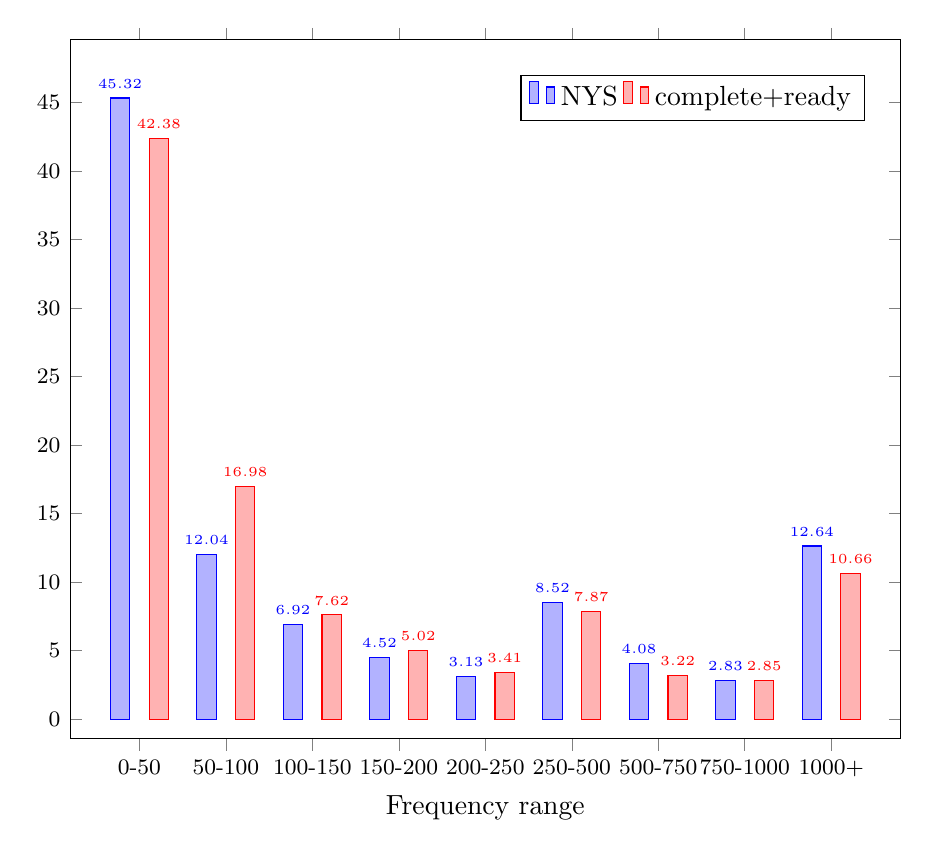
\begin{tikzpicture}[xscale=1.0]
\begin{axis}[
%footnotesize,
width=\textwidth,
    ybar=7pt,bar width=7pt,
%    enlargelimits=0.15,
    legend style={at={(0.75,0.95)},
      anchor=north,legend columns=-1},
    xlabel={Frequency range},
    symbolic x coords={0-50,50-100,100-150,150-200,200-250,250-500,500-750,750-1000,1000+},
    xtick=data,
    nodes near coords,
    nodes near coords align={vertical},
    tick label style = {font = \footnotesize}, %XY LABELS
%    label style = {font = \tiny}, %title below X
%    legend style = {font = \footnotesize},
    every axis plot/.append style = {font = \tiny}
    ]
\addplot coordinates {(0-50,45.3159041394336) (50-100,12.037037037037) (100-150,6.91721132897604) (150-200,4.52069716775599) (200-250,3.1318082788671) (250-500,8.52396514161219) (500-750,4.08496732026144) (750-1000,2.8322440087146) (1000+,12.636165577342) };
\addplot coordinates {(0-50,42.3791821561338) (50-100,16.9764560099133) (100-150,7.62081784386617) (150-200,5.0185873605948) (200-250,3.40768277571252) (250-500,7.86864931846345) (500-750,3.22180916976456) (750-1000,2.85006195786865) (1000+,10.6567534076828) };
\legend{NYS,complete+ready}
\end{axis}
\end{tikzpicture}
\caption{Proportion of NYS and complete and ready verbs w.r.t. frequency range in BNC50.}
\label{fig:04:01}
\end{figure}

\newpage 
At the time of writing, PDEV covered 1,614 verbs for a total of 6,163
patterns, out of an estimated 5,500 total number of verbs in English
(PDEV is therefore about 30\% complete). PDEV is linked to a portion of
the British National Corpus (BNC), BNC50, from which some of the statistics presented in this
chapter are computed. BNC50 contains about 54 million tokens, and BNC,
about 100 million. \figref{fig:04:01} shows that the frequency distribution of
complete verbs is very similar to that of NYS (Not Yet Started) verbs,
e.g. that 40 to 45\% of English verbs have a frequency lower than 50 in
BNC50. For this reason, although PDEV is incomplete, it contains a
representative sample of English verbs, large enough to warrant pilot
studies. Results will need to be confirmed when PDEV is complete.



In PDEV, most verbs have a low number of patterns: the average number of
patterns per verb is 3.8, and the verb with the greatest number of
patterns is \textit{break}, with 83 patterns. More than a
quarter of verbs have only one pattern and 78\% of verbs have five
patterns or less. Verbs can also be contrasted in terms of qualitative
characteristics. Particularly, some of them are used in idioms, others
as phrasal verbs, and others combine with other lexical items in set
phrases, that we propose to call lexically grounded patterns. Table \ref{PDEVcat}
indicates the number of entries and patterns for these MWE-related
categories of verbs.

\begin{table}
%\centering
\begin{tabular}{lrrr}
\lsptoprule
\textbf{MWE type} & \textbf{\# verbs} & \# \textbf{patterns} & \textbf{\% patterns}\\
\midrule
Lexically grounded patterns & 458 & 1,126 & 18.3 \\
Phrasal verb patterns & 198 & 512 & 8.3 \\
Idiom patterns & 200 & 453 & 7.3 \\
\textbf{MWE total} & \textbf{548} & \textbf{1,649} & \textbf{26.7} \\
\lspbottomrule
\end{tabular}
\caption{Number of verbs and of patterns for several MWE categories in PDEV.}
\label{PDEVcat}
\end{table}

















A \textit{lexically grounded pattern} is a pattern
which takes a lexical item or lexical set as an argument, either in
subject, object, complement or adverbial position. For instance
“$[$$[$Human$]$$]$ take \{responsibility\} for $[$$[$Anything$]$$]$” is an example
where a lexical item,  \textit{responsibility}, occupies the object position.
In general the presence of lexical items is a strong sign of fixedness,
so a significant portion of lexically grounded patterns overlap with
idioms. All in all, there are 1,649 MWE patterns in PDEV, which
accounts for 26.7\% of PDEV patterns (about 34\% of verbs). As each
pattern is linked to a set of examples from the BNC, the whole MWE
pattern set is connected to a total of 26,392 corpus examples (an
estimated 84,836 over the whole BNC50, i.e. 1,545 per million).



PDEV \textit{idioms} show very diverse statistical
properties internally. For instance the estimated frequency in BNC
ranges from 1 (e.g.  \textit{blowing off steam}) to 1,071 occurrences (for  \textit{as
follows}) in BNC50, with an average frequency of 23.5 examples in BNC50
and a high standard deviation (67.2). 70\% of idioms have 5 or more
associated examples and 90\% have less than 40 examples. The verb with
the highest number of idioms is \textit{throw}, with 24
idioms. Verbs with idioms on average have, for 64\% of them, one idiom,
for 19\% of them, two idioms, and for 17\%, three or more idioms. 

\section{A CPA study for English-French translation}

The case study presented in this section focuses on  \textit{bite}, because it
was found to encapsulate a large number of facts about English verbs,
and particularly idiomatic structures. This verb is compared to the
French  \textit{mordre}, which translates to `bite' in its primary literal
meaning: `using teeth to cut'. We will observe how these verbs are used
in each language, identify their common features and divergences by
applying CPA to corpora. \textit{Bite} was analysed using a sample of 500
lines from the BNC, and the same sample size was
extracted from the Frtenten corpus (11 billion words; \citealt{jakubicek2013}) for \textit{mordre}.



\textit{Bite} and \textit{mordre} share interesting similarities in terms of their
syntactic and semantic properties. Both verbs are mostly direct
transitive, see examples (\ref{ex7}) and (\ref{ex8}), and can sometimes be accompanied with a
locative adverbial, to indicate the $[$$[$Body Part$]$$]$ bitten. Both verbs
are also used in an intransitive pattern where the bitten entity,
typically found in object position, is moved to a prepositional
complement position, with \textit{into} (\textit{dans} in French) as preposition, see examples (\ref{ex9}) and (\ref{ex10}).



\ea
\label{ex7}
\textit{Those dogs~bit~the neighbours, the dustbin men, visiting aunts and
each other.}
\ex \label{ex8}
\textit{Le propriétaire ou le détenteur d'un chien qui a~mordu~une personne
ou un autre animal a l'obligation de le déclarer au commissariat de son
arrondissement}.
\glt `The owner or the holder of the dog which has bitten a
person or another animal is under the obligation of declaring it to the
district police.'
\ex \label{ex9}
I'll wager that your salivary glands started pumping out liquid as
you imagined yourself~biting~into the lemon.
\ex \label{ex10}
\textit{Je~mords~dans une pêche : un goût d'eau sucrée accompagné d'un
sentiment de vide}.
\glt `I bite in a peach: a taste of sweet water together with a
feeling of emptiness.'
\z





These syntactic patterns are frequently employed in different situations
which sometimes share very little in common with the literal meaning of
the verb. To contrast these uses, CPA entries make use of semantic
types which characterise the semantic properties shared by the
collocates found in a given syntactic slot. In the literal sense of
transitive patterns, \textit{bite} and \textit{mordre} typically collocate with
$[$$[$Human$]$$]$ (with the particular case of vampires) and $[$$[$Animal$]$$]$ (e.g.
\textit{dogs}) as subjects, and with $[$$[$Human$]$$]$, $[$$[$Animal$]$$]$, and $[$$[$Body Part$]$$]$
as objects. Other $[$$[$Physical Object$]$$]$ nouns (e.g. \textit{pillows}, \textit{coins},
\textit{pencils}) were found in English, but not in French, although they
could be found in a larger sample. Transitive patterns of \textit{bite}  were
also found to combine with $[$$[$Eventuality$]$$]$ as subject and $[$$[$Human$]$$]$ or
$[$$[$Institution$]$$]$ as objects, as in example (\ref{ex11}).



\begin{exe}
\ex  \label{ex11} 
\textit{Provincial had been bitten by its own success.}
\end{exe}





In this case, the pattern means “$[$$[$Eventuality$]$$]$ adversely affect
$[$$[$Human$]$$]$ or $[$$[$Institution$]$$]$”. The construction \textit{bite + into} was also
found with a metaphorical pattern expressed as “$[$$[$Event$]$$]$ bites into
$[$$[$Event$]$$]$”, sharing the same meaning as the previous pattern (signaling
an adverse effect). These metaphorical uses of  \textit{bite} seem to be
English-specific: no such pattern was found in the French sample. This
is because French typically uses \textit{ronger} ‘gnaw’, as in example (\ref{ex12}).



\begin{exe}
\ex \label{ex12}
\begin{xlist}
\ex
\textit{The recession is biting deeply into industry.}
\ex
\textit{La recession ronge durement l'industrie.}
\end{xlist}
\end{exe}








When English speakers use \textit{bite} with direct objects such as \textit{nails} or
\textit{fingers} to mean `chewing at one's fingernails, biting the tips off',
French speakers use \textit{ronger} for \textit{ongles} and \textit{doigts} respectively. In
this case, it is also considered as a distinct pattern in French. Other
patterns were found, such as “$[$$[$Physical Object 1$]$$]$ bite in|into
$[$$[$Physical Object 2$]$$]$”,\footnote{English also uses patterns with the
phrasal verb \textit{eat away} for this meaning.} where the subject is
neither $[$$[$Human$]$$]$ nor $[$$[$Animal$]$$]$. This pattern can only be translated
to French with \textit{mordre} to cover uses where “$[$$[$Blade$]$$]$ makes small cuts
into $[$$[$Physical object$]$$]$”. When the subject is \textit{acid}, signalling the
corroding effect the acid has on metal, French uses \textit{ronger}. For other
types of object nouns, such as \textit{ploughs}, French would use the phrasal
expression \textit{se planter} + \textit{dans}.


\largerpage[2]
Semantic types can also help to contrast existing patterns from uses
which combine with specific animals, e.g. $[$$[$Snake$]$$]$, which was found
both in French and English, and which refer to a different situation,
defined as \mbox{“$[$$[$Snake$]$$]$~stabs} \linebreak \mbox{$[$$[$Human$]$$]$~or~$[$$[$Animal$]$$]$~with fangs},
typically injecting poison under the skin”. However, when considering
$[$$[$Insect$]$$]$ (e.g. \textit{mosquitoes}) in subject position, the normal French
verb is \textit{piquer} (see example (\ref{ex13}) below).\footnote{Although \textit{mordu par
les moustiques} is acceptable.}



\begin{exe}
 \ex \label{ex13}
 \begin{xlist}
 \ex 
 \textit{The mosquitos came up and bit me in the dark}.
 \ex
\textit{Les moustiques sont venus et m'ont piqué dans le noir.}
\end{xlist}
\end{exe}





However, \textit{bite} does not collocate with nouns of other flying bugs such
as \textit{wasps}, \textit{bees}, or \textit{hornets},\footnote{English uses the verb \textit{sting}.}
whereas these nouns can be used indifferently with \textit{piquer}. This
language-specific feature can be explained by the extra-linguistic fact
that insects bite to feed, but bees, wasps, and hornets possess a
specific device, positioned at the bottom of their bodies, used to kill
or in self-defence. This is the only pattern where \textit{piquer} can be used
as a translation of \textit{bite}. The pattern “$[$$[$Human$]$$]$ or $[$$[$Animal$]$$]$ bite
through $[$$[$Physical\_Object$]$$]$” also has a literal meaning, but cannot be
translated using \textit{mordre}. The best translation equivalent appears to
be \textit{grignoter} (literally \textit{nibble}), since it keeps the notion of
`using teeth', and correctly translates `insects biting through
leaves'. However this verb does not translate the fact that the bitten
entity is filled with holes. The verb \textit{bite} was only found in a single
intransitive use, “$[$$[$Process$]$$]$ bites”, with the meaning “$[$have$]$ a
noticeable effect, usually an adverse effect”, as in \textit{the recession bit
deeper}. This would be translated into French with the expression \textit{se
faire sentir} (literally `to be felt'). The verb \textit{mordre} was also
found in metaphorical patterns which could not be translated with
\textit{bite}, namely “$[$$[$Building$]$$]$ mord $[$$[$Area$]$$]$”, as in (\ref{ex14}), and
“$[$$[$Vehicle$]$$]$ mord la route”, as in (\ref{ex15}).




%Table 2a - Idiom CPA patterns for the verb ‘\textit{mordre’}




\ea
\label{ex14}
\textit{Certaines des constructions mordaient sur des terres privées}.
\glt `Some of the buildings \textbf{encroached} on private lands.'
\ex \label{ex15}
\textit{Quand vient le temps d'effectuer un dépassement, le véhicule mord
la route}.
\glt `When the time comes to pass the car in front, the vehicle \textbf{grips} the road.'
\z




\begin{table}[b]
\small
%\centering
\begin{tabularx}{\textwidth}{rQrr}
\lsptoprule
No & Pattern / \textit{Implicature} & \parbox{4mm}{\hspace*{-10mm}\mbox{Frequency}} & \%\\
\midrule
4 & $[[[$Human$]]$ | le poisson$]$ mord ($[$à l'hamecon | à l'appat$]$) & 10 & 2\\
%%\midrule
 & \textit{$[$$[$Human$]$$]$ takes the bait (= is lured to do something that has bad consequences)} & & \\
%%\hline
7 & $[[$Human$]]$ mord \{la vie à pleines dents\} & 6 & 1.2\\
%%\midrule
 & \textit{$[[$Human$]]$ enjoys life to the full $[$literally, *bites life with full teeth$]$} & & \\
 %%\midrule
9 & $[[$Human$]]$ se mord \{les doigts\} & 21 & 4.2\\
%%\midrule
 & \textit{$[[$Human$]]$ experiences a bitter time $[$literally, *bites his/her fingers$]$} &  & \\
%%\midrule
11 & $[[$Human 1 $]]$ fait mordre $[$la poussière $]$ $[$à $[[$Human$]]]$ & 6 & 1.2\\
%%\hline
 & \textit{$[[$Human 1 $]]$ causes $[[$Human 2 $]]$ to bite the dust (= to die) or to lose a challenge $[$the latter sense only in French$]$} &  & \\
%%\midrule
12 & $[$le serpent$]$ se mord $[$la queue$]$ & 16 & 3.2\\
%%\midrule
 & \textit{$[[$Human$]]$ is stuck in a $[[$State of affairs$]]$ and cannot find a way out $[$literally, *the snake bites his own tail$]$} &  & \\
%%\midrule
16 & $[[$Human$]]$ ne mord pas $[$NO OBJ$]]$ &
6 & 1.2\\
%%\midrule
 &
\textit{$[[$Human$]]$ does not bite (= is harmless)} &
 &
\\
\lspbottomrule
\end{tabularx}
\caption{Idiom CPA patterns for the verb \textit{mordre}.}
\label{idiom cpa mordre}
\end{table}


\largerpage
In addition to these patterns, 6 idioms were found for \textit{mordre} (see
Table \ref{idiom cpa mordre}), and 10 idioms for \textit{bite} (see Table \ref{idiom cpa bite}).



%Table 2b - Idiom CPA patterns for the verb ‘bit\textit{e’}

%\begin{table}$[$H$]$
%\small
%\centering
%\begin{tabular}{llll}
%%\hline

\begin{table}[t]
\small
%\centering
\begin{tabularx}{\textwidth}{rQrr}
\lsptoprule
No & Pattern / \textit{Implicature} & \parbox{4mm}{\hspace*{-10mm}\mbox{Frequency}} & \%\\
\midrule
13 &
Human 1 bites Human 2's head off &
5 &
1.22\\
%%\midrule
 &
\textit{Human 1 speaks sharply and unkindly to Human 2} &
 &
\\
%%\midrule
14 &
Human bites REFLDET lip &
8 &
1.96\\
%%\midrule
 &
\textit{Human grips his or her lip firmly with the teeth} &
 &
\\
%%\midrule
15 &
Human bites off more than $[$$[$Human$]$$]$ can chew &
4 &
0.98\\
%%\midrule
 &
{\textit{Human undertakes a task that is too difficult for him
or her to accomplish successfully}} &
 &
\\
%%\hline
16 &
Human bites the hand that feeds $[$$[$Human$]$$]$ &
5 &
1.22\\
%%\hline
 &
\textit{Human attacks his or her benefactor} &
 &
\\
%%\hline
17 &
Human or Institution bites the bullet &
21 &
5.13\\
%%\hline
 &
  \mbox{\textit{Human or Institution decides to do something
necessary but unpleasant}} &
 &
\\
%%\hline
18 &
Human is bitten by the $[$MOD$]$ bug &
7 &
1.71\\
%%\hline
 &
\textit{Human becomes very interested in $[$MOD$]$} &
 &
\\
%%\hline
19 &
Human bites the dust &
2 &
0.49\\
%%\hline
 &
\textit{Human dies suddenly and violently} &
 &
\\
%%\hline
20 &
Entity or Process bites the dust &
8 &
1.96\\
%%\hline
 &
\textit{Entity or Process comes to a sudden and unwelcome
end} &
 &
\\
%%\hline
21 &
Human bites REFLDET tongue &
8 &
1.96\\
%%\hline
 &
 \mbox{\textit{Human makes a desperate effort not to say what is on
his or her mind}} &
 &
\\
%%\hline
22 &
Once bitten twice shy &
3 &
0.73\\
%%\hline
 &
\mbox{\textit{An unpleasant experience causes someone to be more
cautious in future}} &
 &
\\
%%\hline
\lspbottomrule
\end{tabularx}
\caption{Idiom CPA patterns for the verb \textit{bite}.}
\label{idiom cpa bite}
\end{table}

  

These idioms share little in common (apart from the correspondence
between patterns 11 in French and 19 in English) and do not involve the
notion of `teeth cutting'. Thus the correct French to English translation
(and vice versa) required knowledge that is encoded in CPA patterns.
Pattern 12, for instance, \textit{le serpent se mord la queue}, is used to
refer to situations where \textit{serpents} ‘snakes’ are not involved, a
phenomenon generally referred to as non-compositionality. In the next
section we propose to measure this property as well as other important
features, such as rigidity, using statistical measures. These measures
will be applied to idioms which will be the focus of  §4.




\section{Statistical measures for the characterisation of MWEs}

In this section, we will describe the use of statistical measures to
automatically characterise the flexibility \is{multiword expression!flexibility} of MWEs. We feel that this
is an important research topic, as it can contribute to describing in
which respects MWEs are flexible and help to speed up their extraction
from corpora.


\subsection{Word association measures and lexicography: PMI}

In psycholinguistics, \textit{word association} means for example that subjects
think of a term such as \textit{nurse} more quickly after the stimulus of a
related term such as \textit{doctor}. \cite{church1989}  redefined \textit{word
association} in terms of objective statistical measures designed to
show whether a pair of words are found together in text more frequently
than one would expect by chance. \is{Point-wise Mutual Information} PMI (Point-wise Mutual Information)
between word x and word y is given by the formula
 
\eabox{\begin{equation*}
I(x,y)=\mathit{log_{2}}P(x,y)/P(x).P(y)
\end{equation*}} 
 
\noindent  where P(x,y) is the probability of the two words occurring in a common
context (such as a window of 5 consecutive words), while $P(x)$ and $P(y)$
are the probabilities of finding words x and y respectively anywhere in
the corpus. PMI is positive if the two words tend to co-occur, 0 if
they occur together as often as one would expect by chance, and less
than 0 if they are in complementary distribution \citep{church1989}.  PMI was used by Church \& Hanks to examine the content word
collocates of the verb \textit{shower}, which were found to include \textit{abuse},
\textit{accolades}, \textit{affection}, \textit{applause}, \textit{arrows} and \textit{attention}. Human
examination of these lists is needed to identify the \textit{seed} members of
categories with which the verb can occur, such as $[$$[$Speech Act$]$$]$ and
$[$$[$Physical Object$]$$]$, giving at least two senses of the verb \citep{hanks2012}. 

\subsection{Span, rigidity, diversity and idiomaticity}

\cite{smadja1993} recommends that collocations should not only be measured
by their \textit{strength}, such as by using the z-score,
but also by their \textit{flexibility}. We propose to
characterise the flexibility of a multiword expression using four
statistical measures, each focusing on a dimension of variation.


A MWE can be characterised by its mean span \textsc{mean span}, that is,
the stretch of text it is found to cover on average. This can be
measured using the mean  $\mu$ of the relative distances between two
words making up the MWE, and computed as follows:
 
\eabox{\begin{equation*}
%µ
\mu \left(X,Y\right)=\frac 1 n\sum _{i=1}^n\mathit{dist}(X_i,Y_i)
\end{equation*}} 




A MWE can also be further characterised by its
\is{rigidity} \textsc{rigidity}. This can be measured using the standard
deviation  $\sigma$ of the relative distances between the two words: 


\eabox{\begin{equation*}
\sigma\left(X,Y\right)=\sqrt{\frac 1 n\sum
_{i=1}^n\left(\mathit{dist}\left(X_i,Y_i\right)-\mu\left(X,Y\right)\right)^2}
\end{equation*}}


For standard deviation, the minimum value when all the examples have
identical span is 0, and there is no theoretical upper limit. Higher
values would indicate a flexible or semantic, rather than a rigid,
lexical collocation.



In a study of David Wyllie’s English translation of Kafka’s
\textit{Metamorphosis}, \cite{oakes2012} found that \textit{stuck fast} and \textit{office
assistant} had mean inter-word distances of 1 with a standard deviation
of 0. This showed that in this particular text, they were completely
fixed collocations where the first word was always immediately followed
by the second. Conversely, \textit{collection} and \textit{samples} had a mean
distance of 2.5 with a standard deviation of 0.25. This collocation was
a little more flexible, occurring both as \textit{collection of samples} and
\textit{collection of textile samples}. \textit{Mr. Samsa} had a mean distance of
1.17 and a standard deviation of 0.32. This is because it usually
appeared as \textit{Mr. Samsa} with no intervening words, but sometimes as
\textit{Mr. and Mrs. Samsa}. 



Another way of looking at the flexibility of a collocation is by
measuring the \is{diversity} \textsc{diversity} of surface forms found for
that collocation. A rigid collocation, where all found examples are
identical in form and span, has very low diversity, while a collocation
which has many surface forms has much higher diversity. One measure of
diversity, popular in ecological studies, is Shannon’s diversity index,
which is equivalent to entropy \is{entropy} in information theory, and given by the
formula:


\eabox{\begin{equation*}
E=-\sum _{i=1}^Np_{i\log _2}p_i
\end{equation*}}





\textit{E} is entropy, \textit{N} is
the number of different surface forms found for the collocation,
\textit{i} refers to each surface form in turn,
and $P_i$ is the proportion of all surface
forms made up of the surface form currently under consideration. The
choice of logarithms to the base 2 ensures that the units of diversity
are bits. The minimum value of diversity (when all the examples of a
MWE are identical) is 0, while the maximum value (when all the examples
occur in different forms) is the logarithm to the base 2 of the number
of examples found.

Finding statistical evidence for the flexibility of a sequence of words
does not automatically entail that all the examples of the sequence
belong to a MWE, and that the reading is non-literal. We therefore
propose to measure the \is{idiomaticity} \textsc{idiomaticity} of a MWE in
context, by taking the ratio of the number of idiomatic occurrences of
the expression divided by its total number of occurrences:


\eabox{\begin{equation*}
\mathit{Idiomaticity}\left(x,y\right)=\frac{\mathit{number}\;\mathit{of}\; \mathit{idiomatic}\; \mathit{occurrences}}{\mathit{total}\; \mathit{number}\; \mathit{of}\; \mathit{occurrences}}
\end{equation*}}


A value of 1 would indicate that the MWE is always idiomatic, while a
lower value would indicate that the MWE can be ambiguous with respect
to its idiomatic reading. It must be borne in mind that this equation
depends on a number of factors such as the overall frequency of the
verb of a MWE in the specific language. The more frequent in everyday
language the constituents of the MWE are, the more probable for them to
be encountered in a corpus in their literal meaning. This is not
related to the idiomaticity of the expression per se, which has to do
with the opacity of the expression: the more opaque (as opposed to
transparent) it is, the more idiomatic it is.


\subsection{Worked out example}

To illustrate how the values of each measure are computed, we propose a
worked out example based on a pair of words used as boundaries, \textit{bite}
and \textit{dog}, in a sample of 10 examples taken from pattern 1 of \textit{bite}:


\ea
"$[$Human 1 | Animal 1$]$ bites $[$Animal 2 | Physical Object | Human 2$]$"
\z


We chose this pair because it is a strong collocation (PMI = 7.7 in
BNC). To apply our statistical measures, the first thing to do is to
compute the distance between the boundary words. First, it is worth
noting that we lump together alternative surface forms of the same
boundary word, so we consider both \textit{dogs} and \textit{dog} as one word.
Different decisions at this stage may lead to different results.


\begin{figure}[b]
%\includegraphics[width=\textwidth]{figures/hankselmaaroufoakesfourth-img002.png}
\begin{tabular}{rlcl}
`A \textcolor{red}{dog}\textsuperscript{-4} that\textsuperscript{-3} barks\textsuperscript{-2} doesn't\textsuperscript{-1} & \textcolor{red}{bite}\textsuperscript{0} & \textcolor{blue}{1} & ,' replied Antonio Navarro, \\
of the \textcolor{red}{dogs}\textsuperscript{-3} that\textsuperscript{-2} had been\textsuperscript{-1} & \textcolor{red}{bitten}\textsuperscript{0} & \textcolor{blue}{2} & and strayed: scared that th \\
in saliva when one animal & \textcolor{red}{bites}\textsuperscript{0} & \textcolor{blue}{3} & another\textsuperscript{1}. in\textsuperscript{2} \textcolor{red}{dogs}\textsuperscript{3} , one of t \\
who had trained his \textcolor{red}{dog}\textsuperscript{-2} to\textsuperscript{-1} & \textcolor{red}{bite}\textsuperscript{0} & \textcolor{blue}{4} & Arabs, and who informed \\
\textcolor{green}{/p$>$$<$p$>$} He was chased and & \textcolor{red}{bitten}\textsuperscript{0} & \textcolor{blue}{5} & by\textsuperscript{1} a\textsuperscript{2} police\textsuperscript{3} \textcolor{red}{dog}\textsuperscript{4} and then a \\
t was saved when her \textcolor{red}{dog}\textsuperscript{-1} & \textcolor{red}{bit}\textsuperscript{0} & \textcolor{blue}{6} & him. \textcolor{green}{$<$/p$><$p$>$} The 22-year- \\
heltenham yesterday after & \textcolor{red}{biting}\textsuperscript{0} & \textcolor{blue}{7} & his\textsuperscript{1} pet\textsuperscript{2} \textcolor{red}{dog}\textsuperscript{3} , which was at \\
time by their own \textcolor{red}{dog}\textsuperscript{-2} are\textsuperscript{-1} & \textcolor{red}{bitten}\textsuperscript{0} & \textcolor{blue}{8} & in the bedroom. In our bree \\
d. \textcolor{green}{$<$/p$><$p$>$} After that \textcolor{red}{dogs}\textsuperscript{-1} & \textcolor{red}{bit}\textsuperscript{0} & \textcolor{blue}{9} & me on the feet. Blood came \\
/ herself that \textcolor{red}{dogs}\textsuperscript{-2} always\textsuperscript{-1} & \textcolor{red}{bite}\textsuperscript{0} & \textcolor{blue}{10} & people, especially them. T
\end{tabular}
\caption{ Example of calculated distances for the pair (\textit{bite}, \textit{dog}) in
concordance for \textit{bite}.}
\label{fig:04:02}
\end{figure}




\figref{fig:04:02} provides an example using signed distance (left or right): in
the first example, \textit{bite} is four words away to the left of \textit{bite}, the
distance is therefore -4. To compute the mean span, however, we
recommend using the unsigned distance (i.e., 4 for the first example),
but it is important to use the signed distance to compute the standard
deviation, in order to capture word order variation. The unsigned text
distances are therefore, in order of appearance of the examples,
4,4,3,2,4,1,3,2,1,2.



The mean  $\mu$ characterises the mean span of an expression: \textit{bite} and
\textit{dog} are 2.6 words apart.


\eabox{\begin{equation*}
\mu_{\left\{\mathit{bite},\mathit{dog}\right\}}=\frac{4+4+3+2+4+1+3+2+1+2}{10}=2.6
\end{equation*}}


The standard deviation characterises the rigidity of an expression and
makes use of the mean of the signed distances  $\mu'$ computed as
follows:


\eabox{\begin{equation*}
\resizebox{11cm}{!}{$
\mu'_{\left\{\mathit{bite},\mathit{dog}\right\}}=\frac{(-4)+(-4)+3+(-2)+4+(-1)+3+(-2)+(-1)+(-2)}{10}=-0.6
$}
\end{equation*}}


The standard deviation can therefore be computed as:


\eabox{\begin{equation*}
\resizebox{11cm}{!}{$\mu^{'}_{\left\{\mathit{bite},\mathit{dog}\right\}}=\sqrt{\frac{\left(-4-\left(-0.6\right)\right)^2+\left(-4-\left(-0.6\right)\right)^2+%\left(3-\left(-0.6\right)\right)^2+%\left(-2-\left(-0.6\right)\right)^2+
…+\left(-2-\left(-0.6\right)\right)^2}{10}}=\sqrt{\frac{76.4}{10}}=2.76$}
\end{equation*}}





The score obtained for \textit{bite} and \textit{dog} is indicative of a low rigidity (2.76).



To compute diversity (entropy), we extract all the patterns of word
forms between boundaries and count the frequency of each pattern class.
Again, characters could also be used as the basic unit, but we use
words; the string of the pattern can be characterised in various ways,
we use word forms. A pattern is a full string between boundaries, with
the null class accounting for cases where boundary words are adjacent.
For X = \{\textit{dog},\textit{dogs}\}, Y = \{\textit{bite},\textit{bites},\textit{bit},\textit{bitten}\}, and i = \{\textit{that
barks doesn’t}, \textit{that had been}, \textit{another. In}, \textit{to}, \textit{by a police},
\{~\}, \textit{his pet}, \textit{are}, \textit{always}\},  $P_i$ corresponds to the number of
times the string is observed in the sample, divided by the total number
of examples (in our case, 10). The entropy is computed as follows:


\eabox{
\resizebox{11cm}{!}{$
E_{\left\{\mathit{bite},\mathit{dog}\right\}}=-\left(\left(\frac
1{10}\log _2\frac 1{10}\right)+\left(\frac 1{10}\log _2\frac
1{10}\right)+…+\left(\frac 1{10}\log _2\frac 1{10}\right)\right)=3.12
$}}


The entropy is quite high as there is no particular pattern that
dominates the sample: only the null pattern occurs twice, but the
others, only once. Finally, no expression formed with \textit{bite} and \textit{dog}
was found to have an idiomatic reading, therefore the idiomaticity is
equal to 0.



The proposed measures are described for two variables. However, many
idioms include more than two words, such as \textit{let the cat out of the
bag}. In such cases we take the span of the idiom as the distance from
the first word to the last, which for this example would be 6 words. 

\section{A contrastive statistical analysis of idioms}

In a pilot experiment on the annotated sample of the BNC corpus of
\textit{bite}, we found that the phrase \textit{bite the bullet} was maximally rigid,
as it occurred all 9 times in exactly that form. Thus the standard
deviation of the collocation span was 0, and its diversity was also 0.
In contrast, the phrase \textit{bitten by the \dots bug} was extremely flexible,
occurring all 6 times in different forms such as \textit{bitten by the travel
bug}, \textit{bitten by the London bug}, and \textit{bitten by the bug of the ocean
floor}. The standard deviation of spans was relatively small (0.48),
reflecting that in all cases but one the variation consisted of the
insertion of a single word, but the diversity index was at its maximum
value for a set of 6 examples, log2(6) = 2.585. 



The results for \textit{bite} were borne out when the experiment was repeated
on a larger corpus, the entire BNC. Table \ref{score idiom bite} shows the results obtained
for English idioms. Idioms are represented by their boundary words and
the table provides the scores using standard measures of collocational
strength (PMI, t-score, and Log-Dice), along with the absolute
frequency and our new measures: \isi{idiomaticity}, \isi{entropy}, \isi{mean span}, and
\isi{standard deviation}.




\begin{table}
\small
%\begin{tabular}{p{1.7cm} p{0.7cm}p{0.7cm}p{0.8cm}p{0.85cm}p{0.85cm}p{0.85cm}p{0.85cm}p{0.9cm}}
\begin{tabularx}{\textwidth}{l@{~}S r@{~~}rQ Q lQ@{~}l}
\lsptoprule
 {Idiom} &
{Freq \mbox{(total)}}  &
 {PMI} &
 {t-score} &
 {Log-Dice} &
{Idioma\-ticity} &
 {Entropy} &
 {Mean\newline  span}  &
 {SD} \\
\midrule
$[$back$]$ $[$bite$]$ &
87 &
5.914 &
10.380 &
5.549 &
0.989 &
0.338 &
1.057 &
0.277\\
%%\hline
$[$bullet$]$ $[$bite$]$ &
36 &
10.484 &
6.477 &
8.561 &
1 &
1.069 &
2.055 &
0.404\\
%%\hline
$[$head$]$ $[$bite$]$ $[$off$]$ &
30 &
6.009 &
7.639 &
5.600 &
0.775 &
3.281 &
3.032 &
2.721\\
%%\hline
$[$dust$]$ $[$bite$]$ &
26 &
8.918 &
5.088 &
7.438 &
1 &
0.235 &
2.03 &
0.192\\
%%\hline
$[$bug$]$ $[$bite$]$ &
19 &
10.589 &
4.688 &
7.894 &
0.842 &
3.326 &
3.125 &
2.578\\
%%\hline
\lspbottomrule
\end{tabularx}
\caption[Summary of scores for some idioms of \textit{bite}.]{Summary of scores for some idioms of \textit{bite}.
SD: Standard Deviation}
\label{score idiom bite}
\end{table}




In the full BNC, there were 19 occurrences of “$[$bite$]$ by X the bug”
altogether, where ``$[$bite$]$'' stands for any grammatical variant of
\textit{bite}, such as \textit{bitten}, and ``X'' stands for any number (possibly zero)
of intervening words. 16 of these were idiomatic, including 3 variants
of the farewell \textit{sleep tight, don’t let the bed bugs bite}, and 3 were
literal as in \textit{I’ve been bitten by bugs in a hooker’s bed}. This gave
an idiomaticity of 16 / 19 = 0.842. Of the idiomatic examples, almost
all were unique, such as \textit{bitten by the travel bug} - the other \textit{bugs}
included \textit{puppy love}, \textit{acting}, \textit{racing}, \textit{flower pressing} and
\textit{showbiz}. On 3 of these occasions the nature of the bug did not appear
between \textit{bitten} and \textit{bug}, which were simply connected as \textit{bitten by
the bug}. The Shannon diversity, resulting from pattern classes of 4, 3
and 3 members and 9 unique occurrences, had a very high value of 3.326.
In terms of rigidity, the mean distance between \textit{bite} and \textit{bug} was
3.125, with a high standard deviation of 2.578. This was because  cases such as \textit{the acting bug really bit me} used the
inchoative alternation, so \textit{bug} appeared before \textit{bit}. Also, influencing rigidity was the fact that even in the active voice, the
number of intervening  words\footnote{Its French adjectival
counterpart, \textit{mordu de} is also  diverse: 
\textit{mordue des nuitées en famille sous la tente} `fanatical about nights
camping with the family', \textit{mordus des jeux on ligne} `addicted to
on-line games' and \textit{mordue d’esperanto} `bitten by the Esperanto
bug.'} could 
vary.



The MWE \textit{bite the bullet} occurred in 36 sentences altogether, there
were no literal examples at all, but that MWE appeared as mentions of
both a racehorse and a pop song. Of the other 34 examples, the vast
majority (29) were exactly in the form “$[$bite$]$ the bullet”, the
remainder being in the forms \textit{bit the ideological bullet} (3), reversed
as in a \textit{harder bullet to bite} (1), and a statement by President Bush
about an opponent: “I bite bullets, he bites nails”. The idiom was
rather rigid, with a mean span of 2.055, and a fairly low standard
deviation of 0.404. Diversity was also low at 1.069. 



The results on French idioms were obtained from the tagged sample from
the Frtenten corpus. The results obtained here have taken only a part
of the corpus into account. In the future, we will perform an
exhaustive analysis of the remaining 196,500 examples. The scores are
given in Table \ref{score idiom mordre}, using the same headers as Table \ref{score idiom bite}.



\begin{table}
\small
\begin{tabularx}{\textwidth}{l@{~}S r@{~~}QS Q l@{~}Q@{~}l}
\lsptoprule
 {Idiom} &
{Freq \mbox{(total)}}  &
 {PMI} &
 {t-score} &
 {Log-Dice} &
{Idioma\-ticity} &
 {Entropy} &
 {Mean\newline  span}  &
 {SD} \\ 
\midrule
$[$poisson$]$ $[$mordre$]$ &
4 &
7.340 &
1.988 &
\mbox{-2.222} &
0.75 &
0 &
1 &
0\\
%%\hline
$[$hameçon$]$ $[$mordre$]$ &
4 &
12.259 &
2 &
2.664 &
0.75 &
0 &
3 &
0\\
%%\hline
$[$appât$]$ $[$mordre$]$ &
2 &
10.475 &
1.413 &
0.894 &
1 &
0 &
3 &
0\\
%%\hline
$[$vie$]$ $[$mordre$]$ &
6 &
4.434 &
2.523 &
-5.126 &
1 &
1.792 &
2.833 &
0.372\\
%%\hline
$[$doigt$]$ $[$mordre$]$ &
21 &
9.387 &
4.789 &
-0.174 &
0.952 &
1.08 &
1.190 &
0.154\\
%%\hline
$[$poussière$]$ $[$mordre$]$ &
6 &
9.360 &
2.446 &
\mbox{-0.204} &
1 &
0 &
1 &
0\\
%%\hline
$[$queue$]$ $[$mordre$]$ &
16 &
9.670 &
4.118 &
0.109 &
1 &
0.34 &
1.187 &
0.527\\
%%\hline
$[$serpent$]$ $[$mordre$]$ &
13 &
11.022 &
3.604 &
1.457 &
1 &
1.7 &
1.846 &
0.591\\
%%\hline
\lspbottomrule
\end{tabularx}
\caption[Summary of scores for some idioms of \textit{mordre} (500 lines sample).]{Summary of scores for some idioms of \textit{mordre} (500 lines sample).
SD: Standard Deviation}
\label{score idiom mordre}
\end{table}



 
The idiom \textit{le poisson mord à l' hameçon} is a popular expression in
French which means `to take the bait' (see Table \ref{idiom cpa mordre}).
As illustrated in
Table \ref{score idiom mordre}, it was found in 3 different forms, which, despite varying mean
span and frequency, were each found to be maximally fixed (standard
deviation = 0) and minimally diverse (entropy~=~0).



The pattern “$[$$[$Human$]$$]$ se mord \{les doigts\}” rarely took its literal
meaning in French, standing for `a person experiencing a bitter time
for his past actions' in 20 cases out of 21. It usually occurred in the
corpus as \textit{mordre les doigts}, but sometimes as \textit{se mord encore les
doigts} `bites his fingers again', \textit{mordrait un peu souvent les
doigts} `bit his fingers a bit often' and other variants. This gave a
mean of 1.19, a standard deviation of 0.15, and an entropy of 1.08.



The idiom \textit{mordre dans la vie à pleine dents} was also found as \textit{mordre
la vie à pleines dents}. Table \ref{score idiom mordre} lists the scores when both variants are
combined. If we consider \textit{vie} as the boundary word (\textit{à pleines dents}
was only found once in a mention of a song), \textit{mordre dans la vie}
occurred 4 times with mean span of 3, while \textit{mordre la vie} was found
twice with mean span of 2.5. Since 5 out of 6 examples had a distance
of 3 words, the standard deviation was quite low (0.372); however the
idiom had a high entropy (2.833), as \textit{mordre la vie} contributed 2
different unique pattern classes to the idiom. 



If we compare English and French, the corresponding phrases \textit{mordre la
poussière} and \textit{bite the dust} both have standard deviations for their
spans of 0, since in the BNC and Frtenten corpora the verb is always
exactly 2 words before the noun. However, as can be seen in Table \ref{idiom cpa mordre},
\textit{mordre la poussière} can have the additional use `losing a challenge'
which was not found in English. The MWEs \textit{bite one's fingers} and its
apparent French translation \textit{se mordre les doigts} are in stark
idiomaticity contrast. While \textit{bite one's fingers} was always found to
be literal (5 cases),~all instances of \textit{se mordre les doigts} (21) were
found to be idiomatic. It is worth noting that translation systems
unaware of these facts will tend to make two mistakes (as can be
checked with Google Translate): when translating from French to
English, they will fail to translate the figurative meaning of \textit{se mordre les doigts} with an equivalent idiom like \textit{kick oneself}. From
English to French, they will fail to translate the literal meaning of
\textit{bite one's fingers} and translate it with the frequent idiomatic
sequence \textit{se mordre les doigts}. For the verbs \textit{mordre} and \textit{bite}, we
have shown that the measures of mean and standard deviation of span,
Shannon Diversity, and idiomaticity give reasonable results as they
reflect the flexibility of a MWE. We could also suggest a measure of
constructional flexibility, which might be the ratio of times a MWE
occurs in the active voice divided by the number of times the MWE
occurs altogether, whether in the active or passive voice.


\section{Generalization of statistical measures}

Evaluating the applicability of statistical measures to different
languages is one way to evaluate their validity. This section describes
other methods to test the generalizability of measures.


\subsection{Comparison with cognitively salient idioms}

\cite[5,21,214]{hanks2013}  makes a distinction between expressions that
are cognitively salient (roughly equivalent to “easily called to mind”)
and socially salient (roughly equivalent to “frequently used”). He
suggests that cognitive salience and social salience are independent
variables, or may even be in an inverse relationship: that is,
frequently used expressions are buried deep in the language user’s
subconscious mind and are not necessarily easily called to mind. The
idioms \textit{kick the bucket} and \textit{spill the beans} are probably the most
cognitively salient and most frequent idioms cited by linguists. Other
idioms cited in this chapter are \textit{grasping at straws}, \textit{the way the
wind blows}, or \textit{shivering in one's boots}. These idioms, along with 4
idioms involving \textit{bite}, make up the set of 10 idioms used for the
experiments described in this section.



In the BNC, \textit{kick the bucket} has 21 occurrences, although another 4
sentences containing both words were discounted as \textit{kick} and \textit{bucket}
appeared in separate clauses. Another 8 were from a linguistic
discussion of the phrase, as in ``notice `kick the bucket' appears as a
verb phrase". Only 5 were idiomatic, in the sense of \textit{to die}: 4 of
these were in the exact form  \textit{kicked the bucket}, while the other had a
sequence of 9 words between \textit{kicked} and \textit{bucket}, in \textit{Arthur kicked
the detonator of the bomb, and consequently the bucket}. This gave a
mean separation of 3.5 words, a standard deviation of 1.870, and a
modest diversity of 0.721. However, these results were biased by a
small sample size and a single creative use of language. This left 8
literal examples of the phrase, as in  \textit{leaving his bucket to be kicked
over by the cow}. Thus idiomaticity was 5/21 = 0.238.

In contrast, the phrase \textit{spill the beans}, found 42 times overall in the
BNC, was almost always (40 times) found in the idiomatic sense of `reveal a secret'. The only exceptions were when the phrase was used as
the title of a book, \textit{A style guide to the New Age called spilling the
beans}, and a television programme \textit{Superchefs spill the beans}, where
the phrase \textit{spill the beans} takes both the literal and the figurative
sense at the same time. The phrase was used just once in its purely
literal sense, where a guest house owner was dreading \textit{a dozen or more
children spilling their beans, wetting the beds, hoarding old crusts}.
Thus idiomaticity was very high: 40/42 = 0.952. Of the 40 idiomatic
cases, the vast majority were in the exact form “$[$spill$]$ the beans”
(37); 2 were in the passive voice (\textit{when the beans are spilled} and
\textit{the beans have been spilled}), and just one replaced \textit{the} with \textit{a
few}: \textit{he spilt a few beans}. The mean separation was 2.025, the
rigidity as measured by the standard deviation was 0.987, and diversity
as measured by entropy was a lowish value of 0.370. According to these
results, \textit{spill the beans} is more idiomatic, less flexible and
slightly less diverse than \textit{kick the bucket}. These findings are in
stark contrast with reports that MWEs like \textit{spill the beans} are more
flexible than the relatively well behaved \textit{kick the bucket}. Although
\textit{kick the bucket} is more idiomatic in the sense that it is fully
opaque, it occurs more often in the text in its literal meaning because
its literal meaning is more frequent in everyday language. 



\begin{table}
\small
\begin{tabularx}{\textwidth}{l@{}S r@{~~}SQ Q l@{~~}Q@{~~}r}
\lsptoprule
 {Idiom} &
{Freq \mbox{(total)}}  &
 {PMI} &
 {t-score} &
 {Log-Dice} &
{Idioma\-ticity} &
 {Entropy} &
 {Mean\newline  span}  &
 {SD} \\ 
\midrule
$[$back$]$$[$bite$]$ &
87 &
5.914 &
10.380 &
5.549 &
0.989 &
0.338 &
1.057 &
0.277\\%\hline
$[$bullet$]$$[$bite$]$ &
36 &
10.484 &
6.477 &
8.561 &
1 &
1.069 &
2.055 &
0.404\\%\hline
$[$head$]$$[$bite$]$ $[$off$]$ &
30 &
6.009 &
7.639 &
5.600 &
0.775 &
3.281 &
3.032 &
2.721\\%\hline
$[$bug$]$$[$bite$]$ &
19 &
10.589 &
4.688 &
7.894 &
0.842 &
3.326 &
3.125 &
2.578\\%\hline
$[$hand$]$$[$bite$]$ $[$BENEFIT$]$ &
15 &
5.584 &
7.639 &
5.196 &
1 &
2.463 &
5.933 &
5.842\\%\hline
$[$bean$]$$[$spill$]$ &
40 &
10.947 &
6.705 &
8.917 &
0.952 &
0.370 &
2.025 &
0.987\\%\hline
$[$straw$]$ $[$grasp/clutch$]$ &
33 &
9.865 &
6.077 &
8.172 &
0.892 &
2.213 &
3.485 &
1.623\\%\hline
$[$way$]$$[$wind$]$ $[$blows$]$ &
21 &
10.663 &
25.264 &
10.652 &
0.676 &
2.488 &
3.5 &
0.534\\%\hline
$[$shoe/boot$]$ $[$quake/shiver  &
12 &
5.043 &
5.056 &
5.608 &
1 &
2.057 &
3.417 &
1.382\\%\hline
/shake$]$ & & & & & & & & \\
$[$bucket$]$$[$kick$]$ &
5 &
8.647 &
4.349 &
7.004 &
0.238 &
0.721 &
3.500 &
1.870\\%\hline
\lspbottomrule
\end{tabularx}
\caption[10 English idioms retained for generalization experiments.]{10 English idioms retained for generalization experiments.\\SD: Standard Deviation}
\label{10 English idioms}
\end{table}


An idiom which stands out in Table \ref{10 English idioms} is \textit{way the wind blows}, which was
by far the strongest collocation according to the t-score and LogDice
measures, and the lowest idiomaticity score (or having the greatest
proportion of literally-intended examples). \textit{bite \ldots bug} had highest
entropy, as one can metaphorically be bitten by many kinds of bug.
Finally \textit{bite \ldots hand \ldots $[$benefit$]$} had the greatest mean span and
standard deviation of span. 


\subsection{Inter-annotator agreement}

Another way of demonstrating the validity of a statistical measure, such
as MWE idiomaticity or mean span, is to determine the \is{inter-annotator agreement} Inter-Annotator
Agreement (or Inter-Rater Reliability, IRR). This is the degree to
which two or more observers might concur on a classification or
annotation task. A measure is only valid to the extent that humans can
agree on the classification of the individual instances which
contribute to the measure. For example, do they agree on whether a MWE
is being used in its idiomatic sense or not, and where it starts and
ends? IRR falls in the range 0 for only random agreement to 1 for
perfect agreement. As an illustration, we estimated the IRR, using
Krippendorff’s $\alpha$ measure,\footnote{Krippendorff’s $\alpha$ may be
calculated using the ‘irr’ package in the R statistical programming
language. The package ‘irr’ can be installed by the following
command: \texttt{install.packages("irr", repos = "http://cran.r-project.org")}

The annotators’
responses should be stored in a matrix, where each row corresponds to
annotators' response values. The R command to create a matrix for three
examples and 2 annotators is, for example: \texttt{m = matrix(c(1,1,3,3,1,2), nrow=2)}.
}
between two native speakers of English
as regards the span and idiomaticity of the phrase \textit{kick the bucket}.
There were 26 sentences in the British National Corpus containing both
\textit{kick} and \textit{bucket}. An $\alpha$ value of 1 denotes perfect agreement
among the annotators, and 0 shows that agreement occurred only by
chance. The instructions given to each annotator were as follows:


\begin{quotation}
For each sentence, choose one of the following:
\end{quotation}

\begin{quotation}
1) the phrase \textit{kick the bucket} (or a grammatical variant of it) does
not appear in the sentence;
\end{quotation}

\begin{quotation}
2) the phrase \textit{kick the bucket} (or a grammatical variant of it) is
idiomatic, and means `to die';
\end{quotation}

\begin{quotation}
3) the phrase \textit{kick the bucket} (or a grammatical variant of it) is
literal, and actually means to physically kick a bucket.
\end{quotation}

\begin{quotation}
If you answered 2) or 3), use $[$ to show where the phrase \textit{kick the bucket} begins and $]$ to show where it ends, as in the example: ``I'm too
young to $[$kick the bucket$]$”.
\end{quotation}


In our experiment to find the agreement of the native speakers as to
whether the phrase \textit{kick the bucket} was absent, literal or idiomatic,
Krippendorff’s $\alpha$ was 0.745.\footnote{Krippendorff’s $\alpha$ is found
by the following command: \texttt{irr:kripp.alpha(m,``nominal").}}  A value
between 0.6 and 0.8 is said to be “good” agreement \citep[404]{altmann1991}.



This experiment was modified to consider only those cases where the
annotators considered the phrase \textit{kick the bucket} to be
present:\footnote{The matrix was modified so that all the 1s (denoting
absence of the phrase) were replaced by “NA” (not applicable).} we were
looking at the agreement between the annotators in distinguishing
literal and idiomatic uses, and Krippendorff’s $\alpha$ was 0.635, still
“good”.



To look at the agreement with respect to the span of the idiom, the
values in the matrix were replaced with the number of words between the
square brackets marked by the annotators, or NA if they did not find
the idiom in the sentence.\footnote{This type of numeric data is called
“ratio” data, so the appropriate command to calculate Krippendorff’s
$\alpha$ is: irr:kripp.alpha(m,``ratio”).} The annotators agreed in every
case where they both marked off the start and end of the idiom ($\alpha$ =
1), showing that the limits of the idiom \textit{kick the bucket} were
clear-cut to these native speakers. Thus according to this small
experiment, the measures of idiomaticity and mean span are valid for
the expression \textit{kick the bucket}. 



\subsection{Correlation and relatedness of measures}

While the previous section illustrated techniques to test the validity
of statistical measures, this section describes a final experiment
focusing on the relatedness of different measures. To do this, we
compared the values of our set of 10 idioms (see Table \ref{10 English idioms}) according to
10 measures. These included the measures of mean and standard deviation
of idiom span, Shannon Diversity and idiomaticity, compared with four
standard measures for collocation strength: \is{frequency!of collocation} frequency of collocation,
PMI, t-score and LogDice. Both the t-score and LogDice are used by the
Sketch Engine lexicographers’ tool \citep{rychly2008}. 



To determine whether these measures were independent of each other or \linebreak
whether one acts as a predictor for another, Spearman’s rank
correlation coefficient was computed for each pair of measures. This
statistic was preferred to the Pearson correlation coefficient, as the
sets of values for some of the individual measures were not normally
distributed. The correlations between the measures are shown in Table
\ref{correlations}. The most statistically significant correlation (p = 0.002, cor =
0.88) was between PMI and LogDice, suggesting that these measures of
collocational strength agree with each other well. Another significant
correlation was the inverse correlation between frequency and mean span
(p = 0.008, cor = -0.78). Thus there was a tendency for more frequent
idioms to be shorter (and to a lesser extent, not statistically
significant) more rigid in their structures. There was no significant
correlation between any of the measures in Table \ref{score idiom bite} and Table \ref{score idiom mordre} with either
of the measures of collocational strength, frequency and PMI.



\begin{table}[ht]
\small
%\begin{tabular}{p{1.8cm}p{0.85cm}p{0.85cm}p{0.85cm}p{0.85cm}p{0.85cm}p{0.8cm}p{0.85cm}p{0.85cm}}
\begin{tabular}{p{1.8cm} r r r r r r r r} 
\lsptoprule
Idiom &
Freq  &
PMI &
t- &
Log- &
Idiom- &
En- &
Mean  &
SD \\
 &
 (total) &
 &
score
 &
Dice &
aticity &
tropy &
span &
 \\
\midrule
Freq &
1 &
~
 &
~
 &
~
 &
~
 &
~
 &
~
 &
~
\\
%\hline
PMI &
0.36 &
1 &
~
 &
~
 &
~
 &
~
 &
~
 &
~
\\
%\hline
t-score &
0.51 &
0.03 &
1 &
~
 &
~
 &
~
 &
~
 &
~
\\
%\hline
LogDice &
0.24 &
\textbf{0.88} &
-0.04 &
1 &
~
 &
~
 &
~
 &
~
\\
%\hline
Idiomaticity &
0.23 &
-0.42 &
-0.09 &
-0.30 &
1 &
~
 &
~
 &
~
\\
%\hline
Entropy &
-0.39 &
0.08 &
0.01 &
0.01 &
-0.29 &
1 &
~
 &
~
\\
%\hline
Mean span &
\textbf{-0.78} &
-0.19 &
-0.15 &
-0.07 &
-0.25 &
0.43 &
1 &
~
\\
%\hline
Standard  &
-0.61 &
-0.27 &
-0.30 &
-0.44 &
-0.20 &
0.62 &
0.55 &
1\\
deviation & & & & & & & & \\
%\hline
\lspbottomrule
\end{tabular}
\caption[Correlations between scores in the 10 idiom study.]{Correlations between scores in the 10 idiom study.\\
SD: Standard Deviation}
\label{correlations}
\end{table}




These results suggest that the new measures of idiomaticity, entropy,
mean span and standard deviation of span may not be useful for
discovering new MWE, but as we have shown, are useful for describing
the characteristics of MWE once discovered. 



\section{Conclusions and perspectives}

\citet{sinclair2004} wrote that the so-called “fixed phrases” are not in fact
fixed: most phrases in English display some variety of form. “Variation
gives the phrase its essential flexibility, so that it can fit into its
surrounding context”. Conversely, each word cannot be considered as a
simple ``Lego brick" which can be fitted in a slot-and-filler system, as
corpus-based investigations reveal that each word preferentially
selects other words, echoing J.R. Firth's maxim that “You should know a
word by the company it keeps”. In this context we have proposed to use
Corpus Pattern Analysis as a technique to describe word patterns found
in corpora, and have applied this technique to two verbs in French and
English. CPA is a corpus-based technique to detect the lexical,
syntactic, and semantic preferences of verbs, such as the fact that
\textit{bite} preferentially selects \textit{mosquitoes} and \textit{bugs} while \textit{sting}
normally selects \textit{bees}, \textit{wasps} and \textit{hornets}. The application of the
CPA methodology to a French corpus revealed however that \textit{mordre}, the
French translation of \textit{bite} in examples such as \textit{dogs bite}, was
neither used with \textit{mosquitoes} nor with \textit{bees}: French speakers prefer
to use \textit{piquer} ‘sting’ for most kinds of ``flying entity aggression".
This suggested that patterns of words are more reliable units of
translation than words in isolation, which opens up new research
perspectives for using CPA in Translation studies and Machine
Translation.



In this chapter, we proposed to use statistical measures which could be
applied to any MWE in any language, by illustration on French and
English. These new statistical measures characterise the flexibility of
a MWE based on text distance: the mean span of MWEs, the standard
deviation of the distance between their boundary words, their internal
diversity, and their idiomaticity ratio. The results obtained by the
application of these measures to \textit{bite} and \textit{mordre} revealed that each
captured useful features of MWEs which compared favourably with
intuitive notions of flexibility and compositionality. It is worth
noting that the implementation of these measures required us to make a number of decisions explicitly, particularly deciding on a
basic unit such as the word or character. Perspectives include testing
these measures on other languages, particularly those with so-called
free word order, and application to Machine Translation.


\largerpage
In his analysis of extended units of meaning, \cite{Sinclair:1991}  noted, as
we have done in our discussion of \textit{bite} and \textit{mordre}, that idioms can
carry across to other languages. In his example, the Italian equivalent
of \textit{naked eye} is \textit{a occhio nudo}. While this is true of many
expressions, the contrastive analysis proposed in this chapter also
suggests that the semantic space occupied by a single lexical item can
be covered by several lexical items in another language. The MWE \textit{naked eye} also exhibits a phenomenon we have not examined in this chapter:
there is greater consistency of patterning to the left of the
collocation than to the right. This suggests that we could use our
measures to find the rigidity or diversity not only of the MWE itself,
but of its context on either side. We could also look for the semantic
prosody associated with MWE – for example, things seen with the naked
eye tend to be difficult (“small”, “weak” or “faint”) to see. 

%\newpage

\section*{Abbreviations}
 
\begin{tabular}{ll}
\textsc{ai} & Artificial Intelligence  \\
\textsc{cpa} & Corpus Pattern Analysis  \\
\textsc{irr} & inter-rater reliability \\
\end{tabular}
\begin{tabular}{ll}
\textsc{pdev} &  Pattern Dictionary of English Verbs  \\
\textsc{pmi} &  Point-wise Mutual Information \\
\textsc{wsd} & Word Sense Disambiguation  \\
\end{tabular} 


%\section*{References}

\sloppy
\printbibliography[heading=subbibliography,notkeyword=this]
%\nocite{*}


\end{document}
